\documentclass[aspectratio=169, 10pt]{beamer}

\usepackage{bm} % bold math
\usepackage{fontspec}
\usepackage{minted}
\usepackage{pgf-pie}
\usepackage{tikz}

% Custom commands and environments
\makeatletter
\newcommand\version[1]{\renewcommand\@version{#1}}
\newcommand\@version{}
\def\insertversion{\@version}

\newcommand\course[1]{\renewcommand\@course{#1}}
\newcommand\@course{}
\def\insertcourse{\@course}

\newcommand\coursetitle[1]{\renewcommand\@coursetitle{#1}}
\newcommand\@coursetitle{}
\def\insertcoursetitle{\@coursetitle}

\newcommand\lecturenumber[1]{\renewcommand\@lecturenumber{#1}}
\newcommand\@lecturenumber{}
\def\insertlecturenumber{\@lecturenumber}
\makeatother

\newcommand{\slidetitle}[1]{{\xbseries \large \structure{#1}} \bigskip}
\newcommand{\term}[1]{{\color{blue} #1}}
\newcommand{\leftspace}{\hspace{1em}}
\newcommand{\inlinearrow}{
  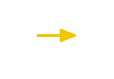
\begin{tikzpicture}[baseline]
    \node [anchor=base] (x) {};
    \draw [rawarrow] (x.mid west) -- ($(x.mid west) + (2em,0)$);
  \end{tikzpicture}
}

\newenvironment{slide}
{\begin{frame}[fragile,environment=slide]\vskip0pt plus 1filll}
{\vskip0pt plus 1filll\end{frame}}

% LaTeX

\setlength{\leftmargini}{1em}

% Common Information

\author{Jon Eyolfson}
\course{ECE 353}
\coursetitle{Systems Software}
\date{2024 Winter}

% fontspec

\defaultfontfeatures{Ligatures=TeX}
% \setmainfont{Domine}
\setsansfont{Inter}[
  FontFace={ul}{n}{Font=*-Thin},
  FontFace={el}{n}{Font=*-ExtraLight},
  FontFace={l}{n}{Font=*-Light},
  FontFace={sb}{n}{Font=*-SemiBold},
  FontFace={eb}{n}{Font=*-ExtraBold},
  FontFace={xb}{n}{Font=*-Black},
]
\setmonofont[Contextuals=AlternateOff, Ligatures=TeXOff]{Iosevka}[
  FontFace={xb}{n}{Font=*-Heavy},
]

%% Font Weights

\DeclareRobustCommand{\ulseries}{\fontseries{ul}\selectfont}
\DeclareTextFontCommand{\textul}{\ulseries}
\DeclareRobustCommand{\elseries}{\fontseries{el}\selectfont}
\DeclareTextFontCommand{\textel}{\elseries}
\DeclareRobustCommand{\lseries}{\fontseries{l}\selectfont}
\DeclareTextFontCommand{\textl}{\lseries}
\DeclareRobustCommand{\sbseries}{\fontseries{sb}\selectfont}
\DeclareTextFontCommand{\textsb}{\sbseries}
\DeclareRobustCommand{\ebseries}{\fontseries{eb}\selectfont}
\DeclareTextFontCommand{\texteb}{\ebseries}
\DeclareRobustCommand{\xbseries}{\fontseries{xb}\selectfont}
\DeclareTextFontCommand{\textxb}{\xbseries}

% tikz

\usetikzlibrary{
  arrows,
  arrows.meta,
  automata,
  backgrounds,
  calc,
  decorations.pathreplacing,
  matrix,
  positioning,
  overlay-beamer-styles,
  shapes,
  shapes.multipart,
  tikzmark,
}

\tikzstyle{rawarrow} = [
  -{Latex[round]},
  line width=1pt,
  yellow,
  shorten >=3pt,
  shorten <=3pt,
  font=\small,
  text=black,
]

\tikzstyle{arrow} = [
  -{Latex[round]},
  line width=1pt,
  yellow,
  shorten >=3pt,
  shorten <=3pt,
  transform canvas={yshift=3pt},
  font=\small,
  text=black,
]

\newcommand{\tikzmarkcoord}[1]{([yshift=3pt]pic cs:#1)}

% minted

\setminted{style=eyolfson, fontsize=\small, escapeinside=||}
\setmintedinline{fontsize=\normalsize}

% hyperref

\hypersetup{colorlinks, urlcolor=blue}

% beamer
\setbeamersize{text margin left=16mm, text margin right=16mm}
\setbeamertemplate{itemize items}[circle]
\setbeamercolor{item}{fg=black}
\setbeamercolor{structure}{fg=darkblue}
\setbeamerfont{frametitle}{series=\bfseries, parent=structure}
\setbeamertemplate{navigation symbols}{}
\setbeamertemplate{headline}{}
\setbeamertemplate{footline}{
  \begin{tikzpicture}[
    remember picture,
    overlay,
    shift={(current page.south west)},
  ]
    \path [fill=gray] (144mm, 0) -- (160mm, 16mm) -- (160mm, 0);
    \node [inner sep=3.5mm, outer sep=0, text=black, anchor=base east,
           align=right, yshift=3.5mm]
          at (current page.south east) {\ttfamily \small \insertframenumber{}};
  \end{tikzpicture}
}
\setbeamertemplate{title page}{
  \begin{tikzpicture}[
    remember picture,
    overlay,
    shift={(current page.south west)},
    background rectangle/.style={fill=darkblue},
    show background rectangle,
  ]
    \node [anchor=center, align=center, text=white, text width=40mm, scale=3.2]
          at (\paperwidth / 2, \paperheight * 2 / 3)
          {\xbseries \inserttitle{}};
    \node [anchor=base west, align=left, inner sep=0, text=white, yshift=2.5mm]
          at (16mm, \paperheight / 3)
          {\insertdate{} \insertcourse{}: \insertcoursetitle{}};
    \node [anchor=base west, align=left, inner sep=0, text=white, yshift=-2.5mm]
          at (16mm, \paperheight / 3)
          {\insertauthor};
    \node [anchor=base east, align=right, inner sep=0, text=white, yshift=2.5mm]
          at (144mm, \paperheight / 3)
          {Lecture \insertlecturenumber{}};
    \node [anchor=base east, align=right, inner sep=0, text=white,
           yshift=-2.5mm]
          at (144mm, \paperheight / 3)
          {\ttfamily \insertversion{}};
    \node [align=center, anchor=south, inner sep=0, text=white, yshift=3.5mm]
          (license) at (\paperwidth / 2, 0)
          {\fontsize{7pt}{7pt}\selectfont This  work is licensed under a
           \href{http://creativecommons.org/licenses/by-sa/4.0/}
                {\color{lightblue} Creative Commons Attribution-ShareAlike 4.0
                 International License}};
  \end{tikzpicture}
}

% xcolor

%% Primary Colour

\definecolor{pantone655}{RGB}{0, 42, 92} % #002a5c
\colorlet{darkblue}{pantone655}

%% Secondary Colours

\definecolor{pantone633}{RGB}{0, 139, 176} % #008bb0
\colorlet{blue}{pantone633}

\definecolor{pantonewarmred}{RGB}{220, 70, 51} % #dc4633
\colorlet{red}{pantonewarmred}

\definecolor{pantone3285}{RGB}{0, 161, 137} % #00a189
\colorlet{cyan}{pantone3285}

\definecolor{pantone7722}{RGB}{13, 83, 77} % #0d534d
\colorlet{darkcyan}{pantone7722}

\definecolor{pantone376}{RGB}{141, 191, 46} % #8dbf2e
\colorlet{green}{pantone376}

\definecolor{pantone2613}{RGB}{109, 36, 122} % #6d247a
\colorlet{violet}{pantone2613}

\definecolor{pantone2985}{RGB}{111, 199, 234} % #6fc7ea
\colorlet{lightblue}{pantone2985}

\definecolor{pantone227}{RGB}{171, 19, 104} % #ab1368
\colorlet{magenta}{pantone227}

\definecolor{pantone7406}{RGB}{241, 197, 0} % #f1c500
\colorlet{yellow}{pantone7406}

%% Neutrals

\definecolor{pantonecoolgray2}{RGB}{208, 209, 201} % #d0d1c9
\colorlet{gray}{pantonecoolgray2}


\lecturenumber{20}
\title{Locks}
\version{2.0.0}

\begin{document}
  \begin{frame}[plain, noframenumbering]
    \titlepage
  \end{frame}

  \begin{slide}

    \slidetitle{Data Races Can Occur When Sharing Data}

    A data race is when two concurrent actions access the same variable

    and at least one of them is a write operation

  \end{slide}

  \begin{slide}

    \slidetitle{Atomic Operations are Indivisible}

    Any atomic instruction you may assume happens all at once
    \medskip

    This means you can not preempt it
    \medskip

    However, between two atomic instructions, you may be preempted

  \end{slide}

  \begin{slide}

    \slidetitle{Three Address Code (TAC) is Intermediate Code Used by Compilers}

    TAC is mostly used for analysis and optimization by compilers
    \medskip

    Statements represent one fundamental operation (assume each is atomic)

    \leftspace{}Useful to reason about data races and easier to read than assembly
    \medskip

    Statements have the form: $result := operand_1\:operator\:operand_2$

  \end{slide}

  \begin{slide}

    \slidetitle{GIMPLE is the TAC used by \texttt{gcc}}

    To see the GIMPLE representation of your compilation use:

    \leftspace{}{\tt -fdump-tree-gimple} flag
    \medskip

    To see all the three address code generated by the compiler (gcc) use:

    \leftspace{}{\tt -fdump-tree-all} flag
    \medskip

    GIMPLE is easier to reason about your code at a low-level without assembly

  \end{slide}

  \begin{slide}

    \slidetitle{\texttt{17-threads-implementation/pthread-datarace.c} Data Race}

    Instead of \texttt{count}, we'll look at \texttt{pcount} (the pointer to
    count, which is a global)
    \medskip

    The GIMPLE is the following:
    \begin{minted}{c}
D.1 = *pcount;
D.2 = D.1 + 1;
*pcount = D.2;
    \end{minted}
    \medskip
    
    Assuming that two threads execute this once each
    and initially \texttt{*pcount = 0}

    \leftspace{}What are the possible values of \texttt{*pcount}?

  \end{slide}

  \begin{slide}

    \slidetitle{
      To Analyze Data Races, You Have to Assume All Preemption Possibilities
    }

    Let's call the read and write from thread 1 R1 and W1 (R2 and W2 from thread 2)
    \medskip

    We'll assume no re-ordering of instructions: always read then write in
    a thread
    \medskip

    All possible orderings:

    \begin{center}
      \begin{tabular}{llll|r}
        \multicolumn{4}{c|}{Order} & {\tt *pcount}\\
        \hline
        R1 & W1 & R2 & W2 & 2 \\
        R1 & R2 & W1 & W2 & 1 \\
        R1 & R2 & W2 & W1 & 1 \\
        R2 & W2 & R1 & W1 & 2 \\
        R2 & R1 & W2 & W1 & 1 \\
        R2 & R1 & W1 & W2 & 1 \\
      \end{tabular}
    \end{center}

  \end{slide}

  \begin{slide}

    \slidetitle{You Can Create Mutexes Statically or Dynamically}

    \begin{minted}{c}
pthread_mutex_t m1 = PTHREAD_MUTEX_INITIALIZER;
pthread_mutex_t m2;

pthread_mutex_init(&m2, NULL);
...
pthread_mutex_destroy(&m1);
pthread_mutex_destroy(&m2);
    \end{minted}
    \medskip

    If you want to include attributes, you need to use the dynamic version

  \end{slide}

  \begin{slide}

    \slidetitle{Everything Within the Lock and Unlock is a Critical Section}

    \begin{minted}{c}
// code
pthread_mutex_lock(&m1);
// protected code
pthread_mutex_unlock(&m1);
// more code
    \end{minted}
    \medskip

    Everything within the {\tt lock} and {\tt unlock} is protected
    \medskip

    Be careful to avoid deadlocks if you are using multiple mutexes
    \medskip

    There's also a {\tt pthread\_mutex\_trylock} if needed

  \end{slide}

  \begin{slide}

    \slidetitle{Adding a Lock to Prevent the Data Race}

    \begin{minted}{c}
static pthread_mutex_t mutex = PTHREAD_MUTEX_INITIALIZER; /* New */
static int counter = 0;

void* run(void* arg) {
    for (int i = 0; i < 100; ++i) {
        pthread_mutex_lock(&mutex); /* New */
        ++counter;
        pthread_mutex_unlock(&mutex); /* New */
    }
}

int main(int argc, char *argv[])
{
    // Create 8 threads
    // Join 8 threads
    pthread_mutex_destroy(&mutex); /* New */
    printf("counter = %i\n", counter);
}
    \end{minted}

  \end{slide}

  \begin{slide}

    \slidetitle{A Critical Section Means Only One Thread Executes Instructions}

    Safety (aka mutual exclusion)

    \leftspace{}There should only be a single thread in a critical section at
    once
    \medskip

    Liveness (aka progress)

    \leftspace{}If multiple threads reach a critical section, one must proceed

    \leftspace{}The critical section can't depend on outside threads

    \leftspace{}\leftspace{}You can mess up and deadlock (threads don't make progress)
    \medskip

    Bounded waiting (aka starvation-free)

    \leftspace{}A waiting thread must eventually proceed

  \end{slide}

  \begin{slide}

    \slidetitle{Critical Sections Should Also Have Minimal Overhead}

    Efficient

    \leftspace{}You don't want to consume resources while waiting
    \medskip

    Fair

    \leftspace{}You want each thread to wait approximately the same time
    \medskip

    Simple

    \leftspace{}It should be easy to use, and hard to misuse

  \end{slide}

  \begin{slide}

    \slidetitle{Similar to Libraries, You Want Layers of Synchronization}

    \centering
    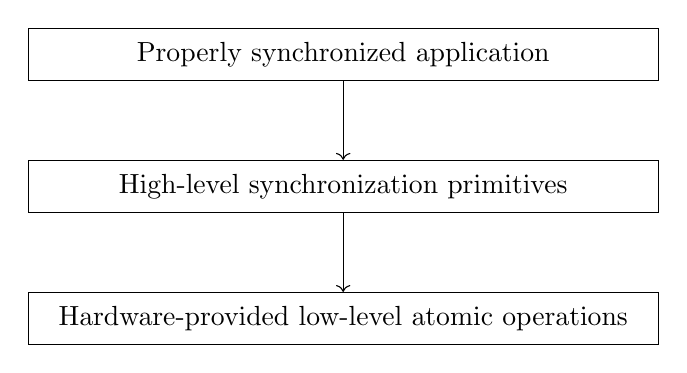
\begin{tikzpicture}[every node/.style={draw, minimum width=8cm, inner sep=0.5em}]
      \node (app) {Properly synchronized application};
      \node [below=of app] (hl) {High-level synchronization primitives};
      \node [below=of hl] (hw) {Hardware-provided low-level atomic operations};
      \draw [->] (app) -- (hl);
      \draw [->] (hl) -- (hw);
    \end{tikzpicture}

  \end{slide}

  \begin{slide}

    \slidetitle{You Could Use a Lock to Implement Critical Sections}

    Assuming a uniprocessor operating system, your implementation could be:
    \medskip

    \begin{minted}{c}
void lock() {
  disable_interrupts();
}
void unlock() {
  enable_interrupts();
}   
    \end{minted}
    \medskip

    This would disable concurrency (assuming it ignores signals and interrupts)

    \leftspace{}This does not work on multiprocessors

  \end{slide}

  \begin{slide}

    \slidetitle{Let's Try to Implement a Lock in Software}

    \begin{minted}{c}
void init(int *l) {
  *l = 0;
}
void lock(int *l) {
  while (*l == 1);
  *l = 1;
}
void unlock(int *l) {
  *l = 0;
}   
    \end{minted}
    \medskip

    What's the issue with this implementation?

    \onslide<2->{\leftspace{}It's not safe (both threads can be in the critical section)}

    \onslide<2->{\leftspace{}It's not efficient, it wastes CPU cycles (busy wait)}

  \end{slide}

\end{document}
